\section{Supporting differentiability experiments}
\label{app:differentiability-support}

\subsection{Finite-difference step dependence}
\label{app:gradient-fd}

Figure~\ref{fig:gradient-fd} shows the relative discrepancy between the
reverse-mode derivatives of Table~\ref{tab:gradient-verification} and centred
finite differences as a function of the perturbation magnitude. The broadly
flat errors for the temperature and LAI controls and the shallow optimum for
soil water are consistent with a resolved centred-difference approximation in
double precision.

\begin{figure}[H]
\centering
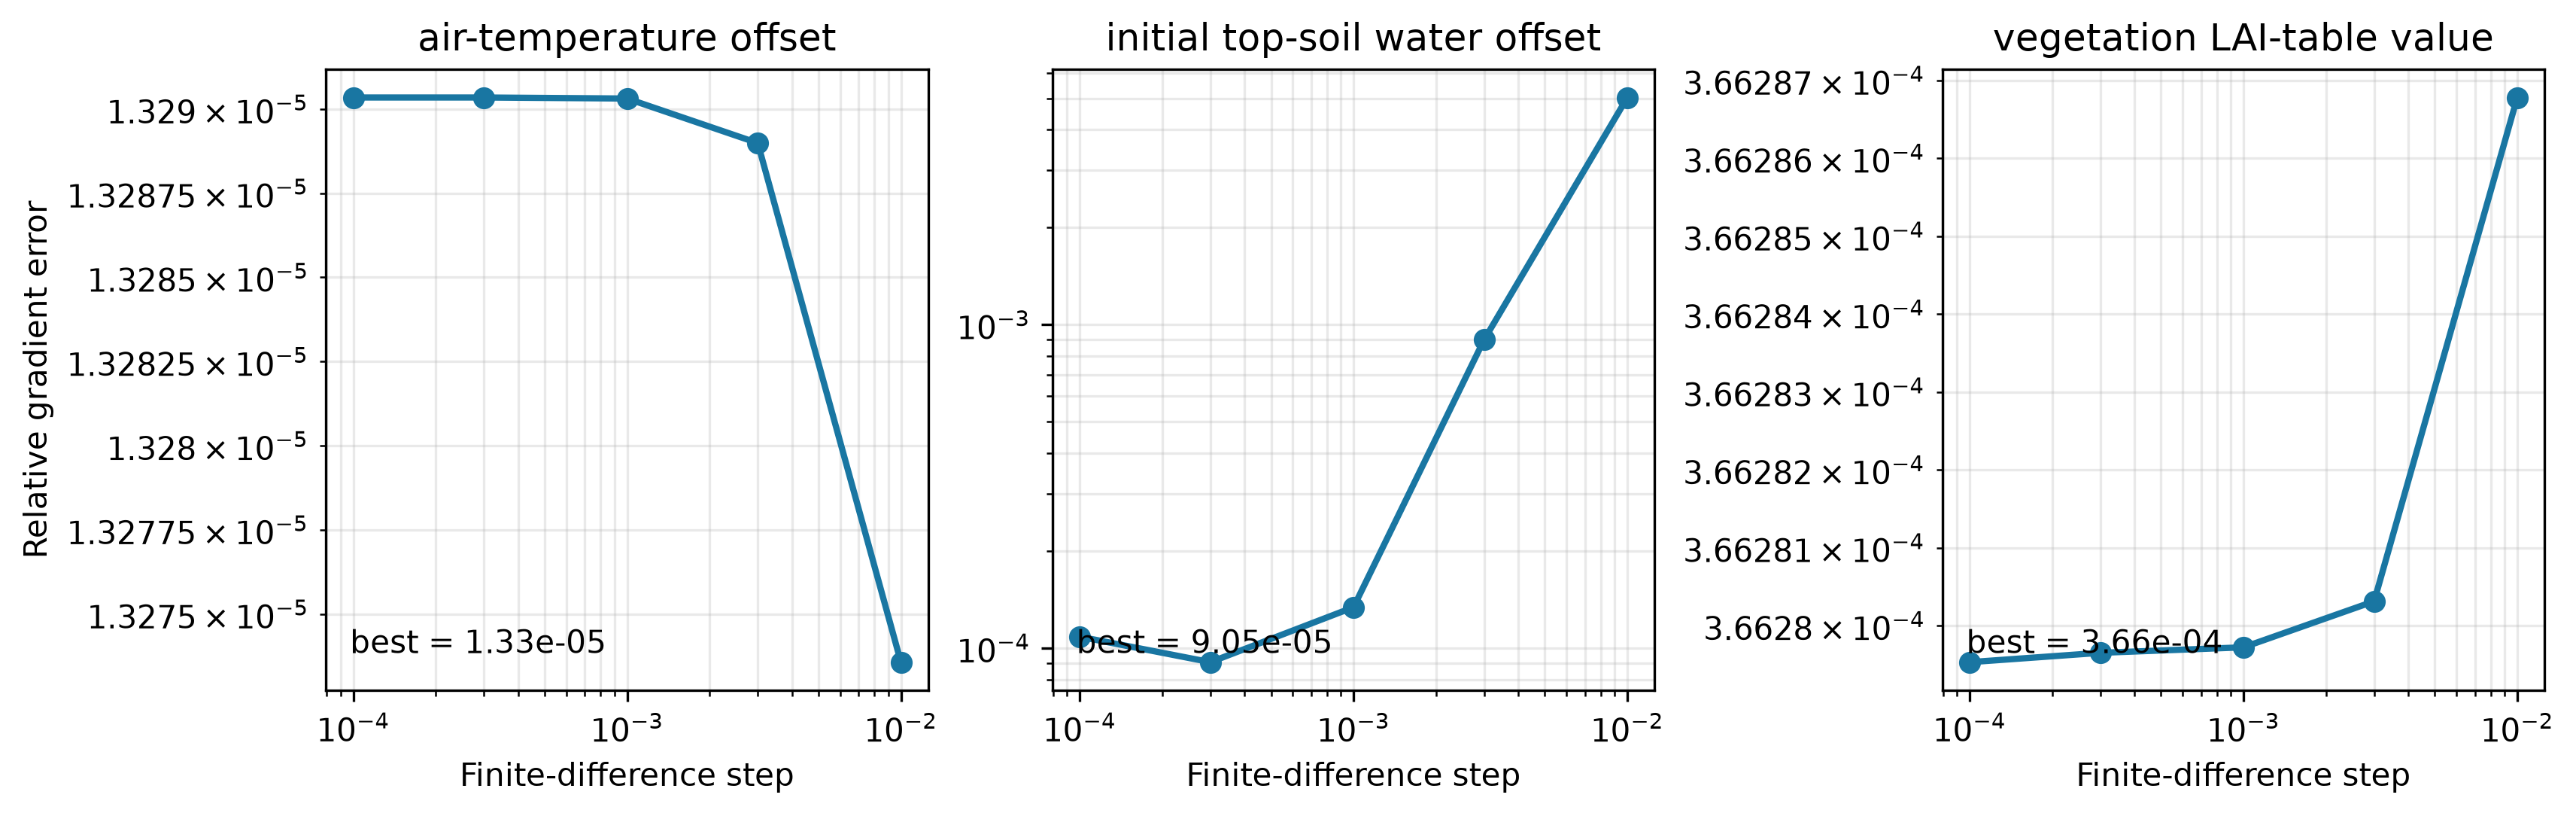
\includegraphics[width=\linewidth]{figures/gradient_finite_difference_check.png}
\caption{Relative discrepancy between reverse-mode automatic derivatives and
centred finite differences for the 24~h SURF trajectory. Each panel uses the
same loss and control as the corresponding row in
Table~\ref{tab:gradient-verification}.}
\label{fig:gradient-fd}
\end{figure}

\begin{figure}[H]
\centering
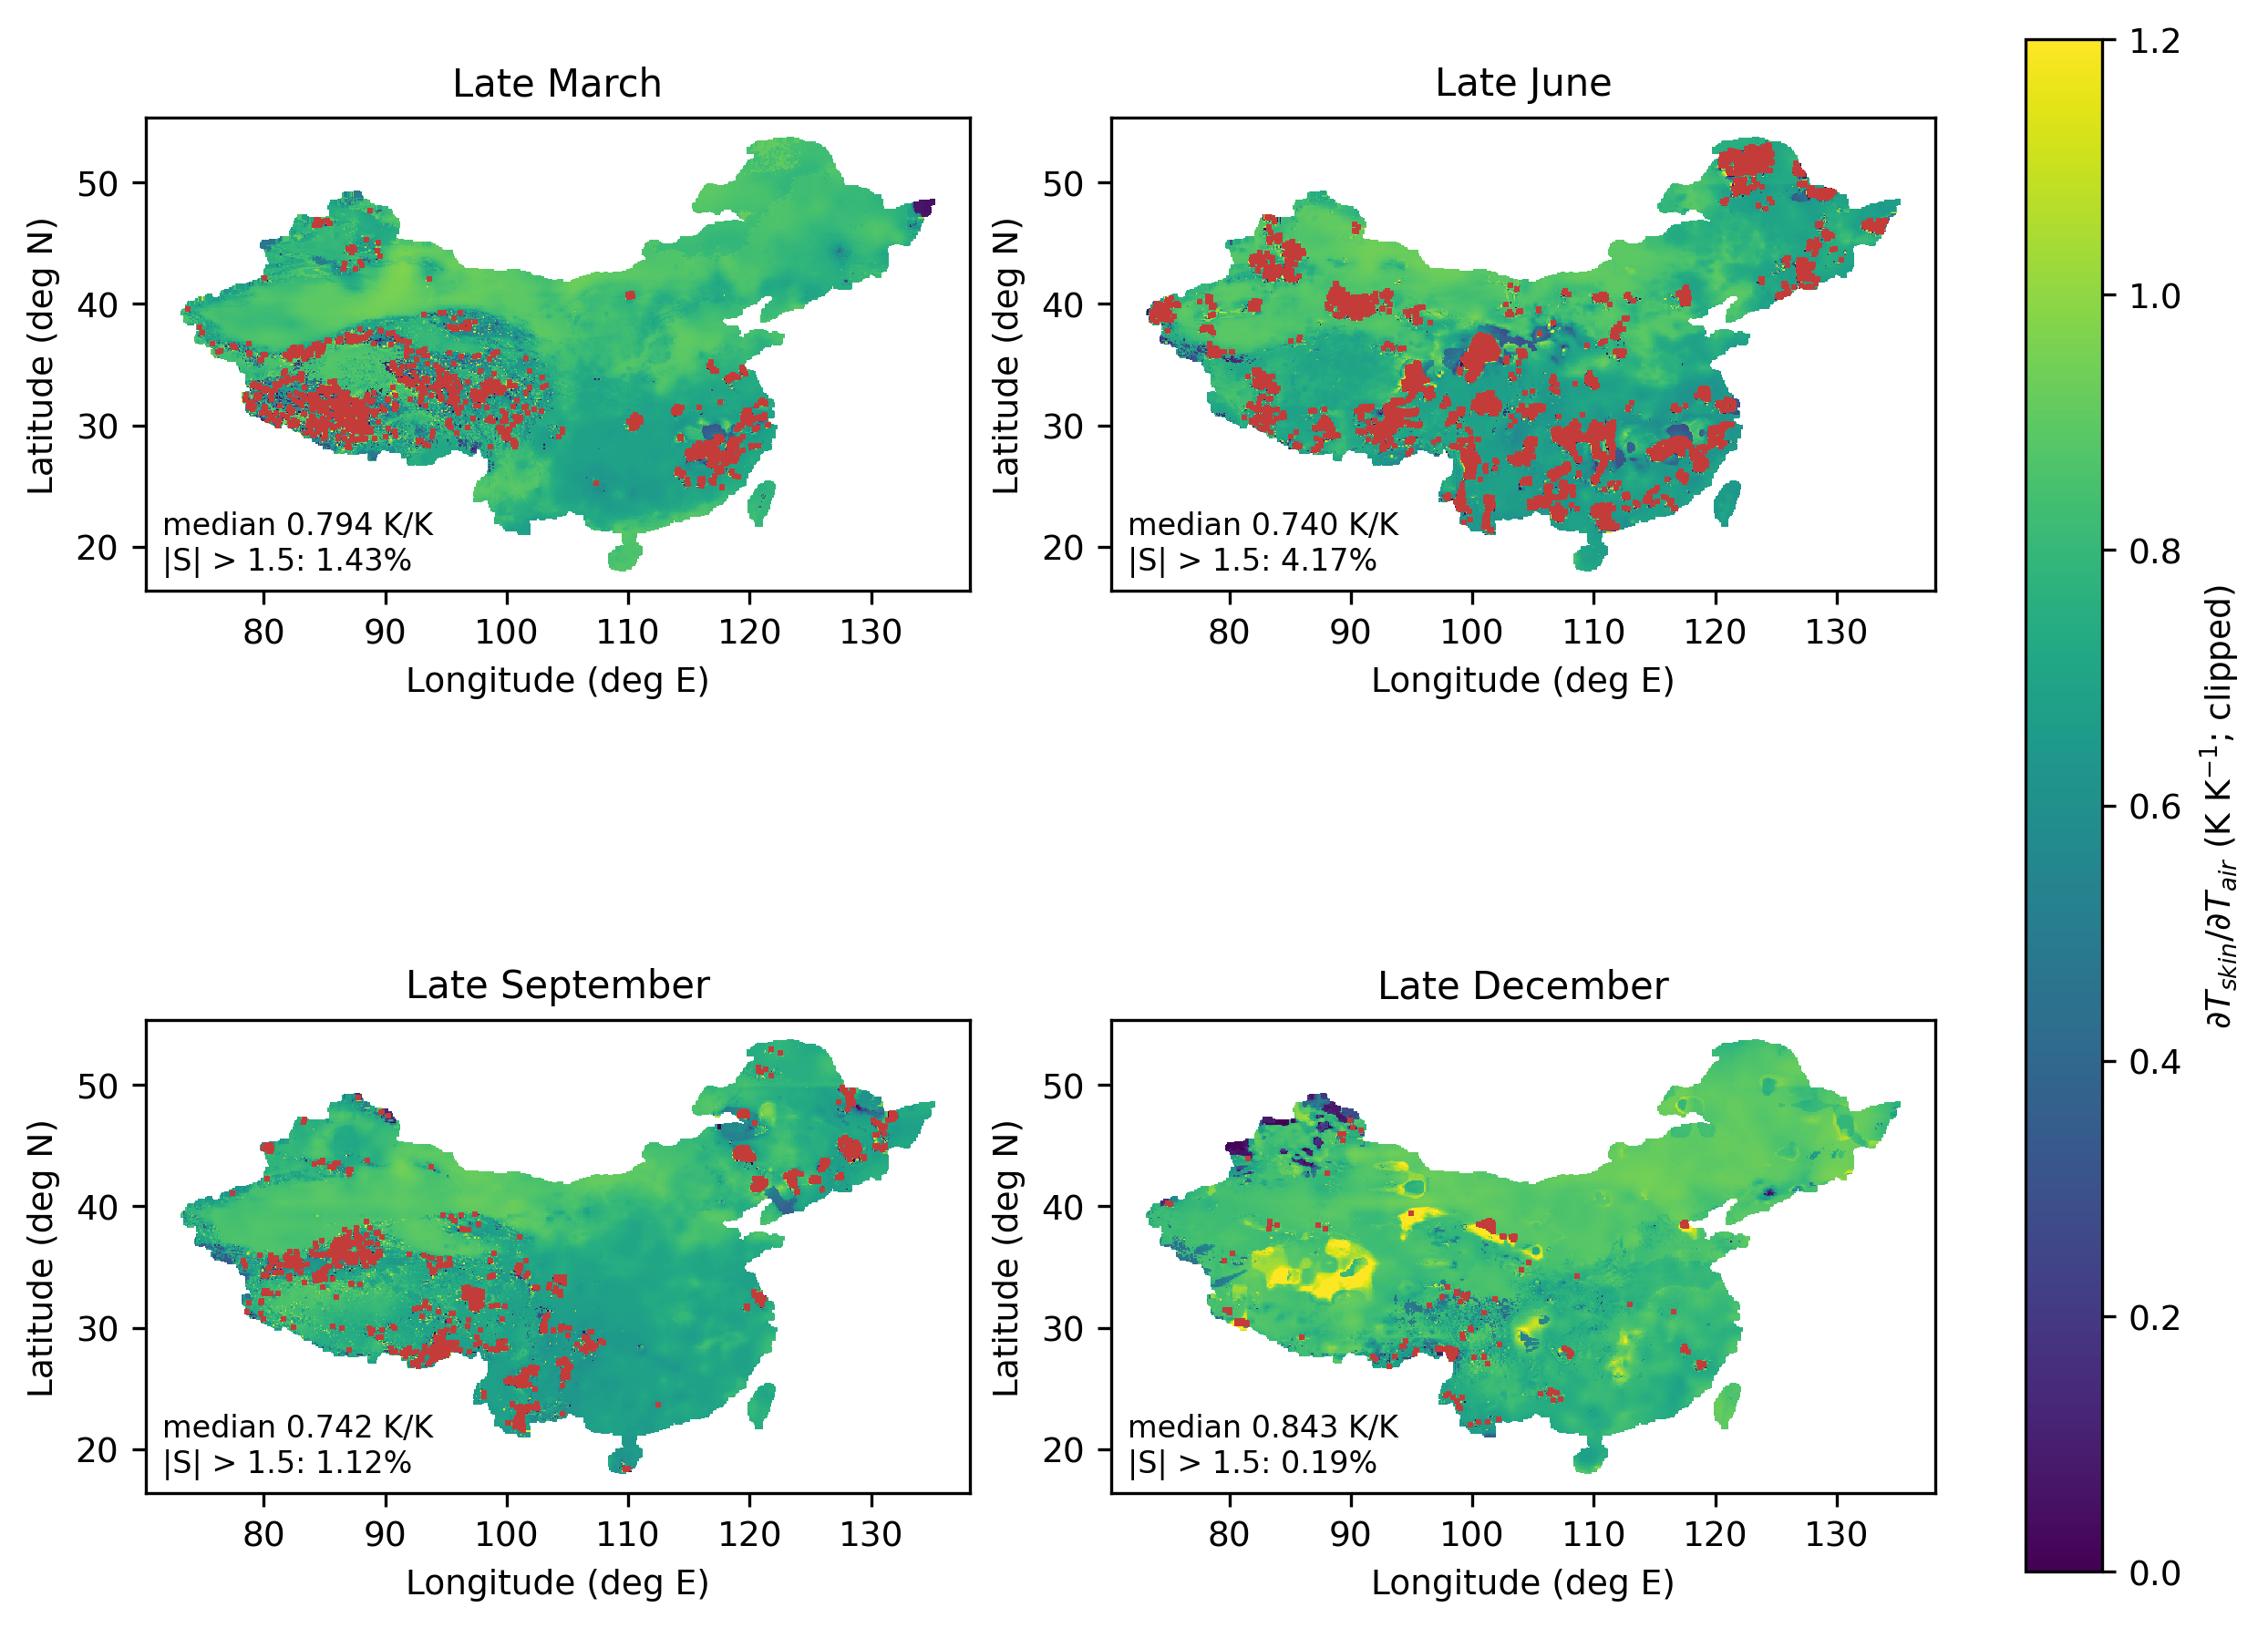
\includegraphics[width=\linewidth]{figures/seasonal_tair_sensitivity_maps.png}
\caption{Seasonal local response of terminal skin temperature to an
independent near-surface air-temperature offset, calculated by reverse-mode
automatic differentiation over a 6~h CMFD window following a 24~h unperturbed
closure adjustment. Colours show $\partial T_{\rm skin}/\partial T_{\rm air}$
between 0 and 1.2~K~K$^{-1}$; red pixels mark the separately reported
threshold-sensitive columns with an un-clipped absolute response above
1.5~K~K$^{-1}$.}
\label{fig:seasonal-tair-sensitivity}
\end{figure}

\subsection{Fortran-guided initial-state retrieval}
\label{sec:fortran-guided-retrieval}

The verified derivative also admits an inverse calculation against an
independent target. The target trajectory is the separately executed Fortran
offline integration of the autonomous CMFD experiment, rather than a PyTorch
synthetic twin. A representative warm, snow-free column at
$23.05^\circ$~N, $107.55^\circ$~E was selected from the Fortran day-10 and
day-20 states alone using a fixed median-state rule; the day-10 values of
top- and second-layer soil water and top-layer soil temperature form the
calibration target, and the day-20 state is held out for validation.
Starting from the common restart with a known $+5.0$~kg~m$^{-2}$
perturbation of the initial top-layer soil water, the residual
$r_i(d)=[h_i(d)-y_{{\rm F},i}]/s_i$ (scales $s_i$ of 5 and
10~kg~m$^{-2}$ and 1~K) is minimized with a damped Gauss--Newton update whose
Jacobian is obtained by reverse-mode automatic differentiation through the
full 10-day trajectory; no finite-difference integrations enter the update.

Five updates reduced the imposed bias from 5.0 to 0.170~kg~m$^{-2}$
(Fig.~\ref{fig:fortran-guided-retrieval}); at day~10 the absolute errors of
the three calibrated variables decreased by 93.9--95.9~\%, and the held-out
day-20 Fortran state independently confirms a 96.1--96.2~\% reduction for all
three variables (Table~\ref{tab:fortran-guided-retrieval}). The unperturbed
common restart remains a numerical reference, with day-10 differences below
$3.23\times10^{-6}$~kg~m$^{-2}$ and $1.21\times10^{-5}$~K, so the retrieval
does not conceal a structural Fortran--PyTorch offset; it recovers a
prescribed initial-condition error using a target external to the
differentiated model. The experiment is a process-level demonstration rather
than an observation-assimilation result; extending it will require observation
operators, uncertainty models, and multi-column controls.

\begin{table}[H]
\caption{Absolute PyTorch errors relative to the Fortran initial-state
retrieval target. The day-10 values enter the Gauss--Newton objective; the
day-20 values are held out. ``Biased'' is the prescribed $+5.0$~kg~m$^{-2}$
initial top-soil-water perturbation, and ``retrieved'' is the state after five
updates.}
\label{tab:fortran-guided-retrieval}
\centering
\small
\begin{tabular}{lrrrr}
\hline
Quantity (unit) & day-10 biased & day-10 retrieved & day-20 biased & day-20 retrieved \\
\hline
Soil water, layer 1 (kg m$^{-2}$) & $4.04\times10^{-1}$ & $1.64\times10^{-2}$ & $3.01\times10^{-1}$ & $1.17\times10^{-2}$ \\
Soil water, layer 2 (kg m$^{-2}$) & $1.15$ & $4.70\times10^{-2}$ & $6.88\times10^{-1}$ & $2.64\times10^{-2}$ \\
Soil temperature, layer 1 (K) & $2.68\times10^{-3}$ & $1.62\times10^{-4}$ & $1.28\times10^{-2}$ & $4.89\times10^{-4}$ \\
\hline
\end{tabular}
\end{table}

\begin{figure}[H]
\centering
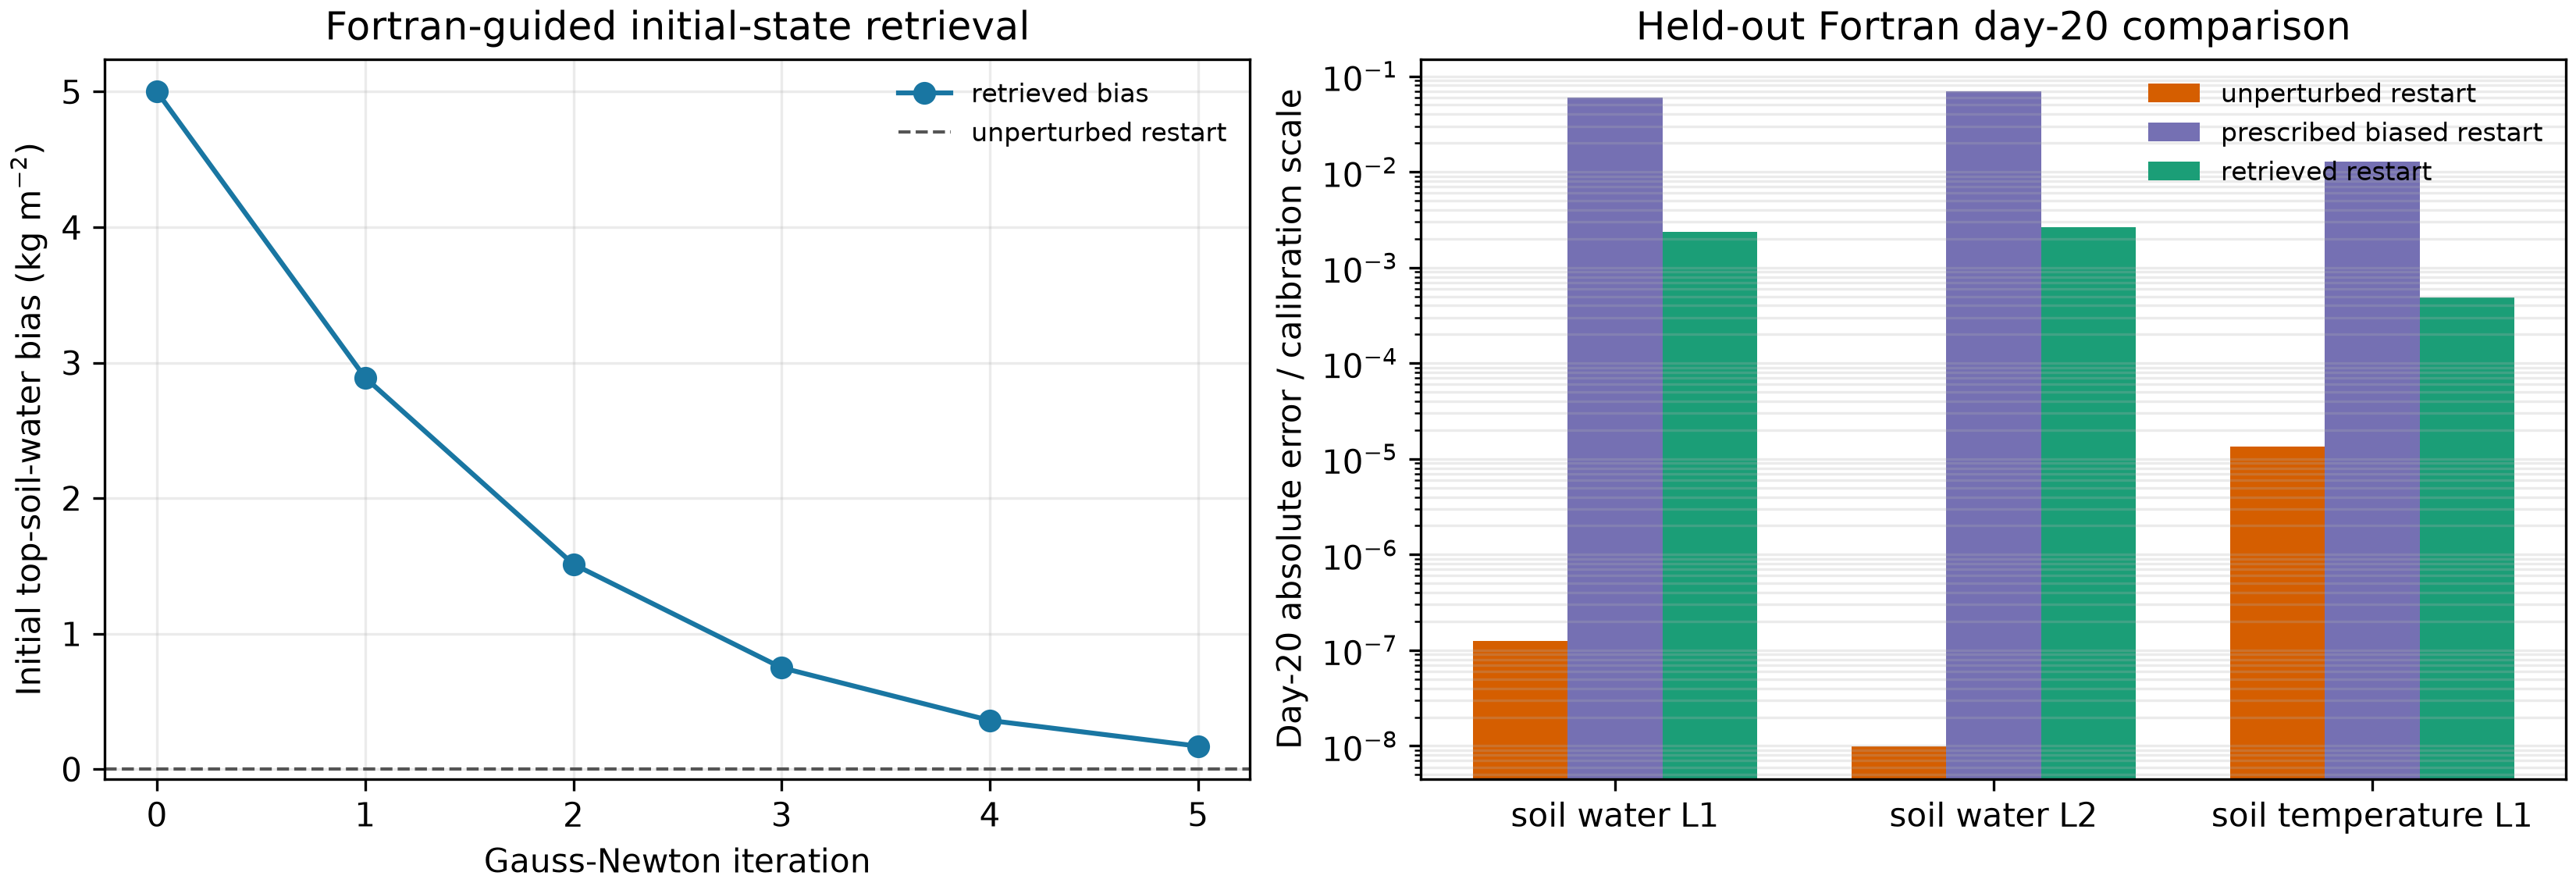
\includegraphics[width=\linewidth]{figures/fortran_guided_initial_state_inversion.png}
\caption{Fortran-guided initial-state retrieval using an autonomous offline
SURF trajectory. Left: reverse-mode, damped Gauss--Newton recovery of the
prescribed top-layer soil-water bias from the day-10 Fortran target. Right:
normalized absolute errors against the held-out day-20 Fortran state. The
unperturbed restart is shown only as a numerical-reference path and is not
used to construct the retrieval target.}
\label{fig:fortran-guided-retrieval}
\end{figure}
